\documentclass[12pt,a4paper]{report}
% importation des packages
\usepackage[utf8]{inputenc}
\usepackage[francais]{babel}
\usepackage{graphicx}
\graphicspath{ {./images/} }
\usepackage{subcaption}
\usepackage{wrapfig}


%hauts et bas de pages
\usepackage{fancyhdr}
\usepackage{color}
\usepackage[dvipsnames]{xcolor}
\usepackage[Glenn]{fncychap}
\pagestyle{fancy}
\lhead{Projet de Science des données}
\rhead{Groupe SantEconomie} 
\lfoot{License MIASHS}
\rfoot{2022/2023} 
\cfoot{\textbf{Page \thepage}}
\renewcommand{\headrulewidth}{1pt}
\renewcommand{\footrulewidth}{1pt}

% Définition du format pour le chapitre pour le mettre en couleur à modifier 
%\titleformat{\chapter}[display]
  %{\normalfont\Large\bfseries\color{myblue}}
  %{\chaptertitlename\ \thechapter}{20pt}{\Huge}

\begin{document}

%------------------------------------------------premiere page
\begin{titlepage}

%logo paul valéry et logo projet
\begin{center}
\begin{figure}[h]
    \centering
    \begin{subfigure}{0.3\textwidth}
        \centering
        
\includegraphics[width=\linewidth]{images/Logo_univ.png}
    \end{subfigure}
    \hspace{3cm}
    \begin{subfigure}{0.4\textwidth}
        \centering
        
\includegraphics[width=\linewidth]{images/Logo_SanEconomie.png}
    \end{subfigure}
    \label{fig:images}
\end{figure}

\medskip
{\Large{Universit\'{e} Paul Val\'{e}ry }}\\
\textsc{UFR 6}\\
 \vskip0.5cm
  \noindent {\textsc{\LARGE \textcolor{MidnightBlue}{Licence MIASHS}}\\[1cm]}
\end{center}
\vskip0.5cm
\begin{center}
\textbf{Projet de science des donn\'{e}es}\\
\vskip0.5cm
%------------------------------------------------
\newcommand{\HRule}{\rule{\linewidth}{0.5mm}} 
	\HRule\\[0.2cm]
	{\huge\bfseries\textcolor{MidnightBlue}{Projet SantEconomie\\[0.2cm]}}
	\HRule\\[1cm]
%------------------------------------------------
Par: \\
\small \bf{\ Girondin Audric, Can Arisoy Ivan, Duckes Jonathan, \\ Carot-Gelas Axel, Ravalisaona Malala, Abdallah Rachydah}
\end{center}
%------------------------------------------------
  \vspace{3mm}
  \centerline {\small \bf{\ Soutenue le $03/05/2022$}}
  \vspace{3mm}
  \centerline {\small \bf{\ Encadrants : $Sandra Bringay, Namrata Patel$}} 
%------------------------------------------------
\vskip2.5cm
\begin{center}
{\small{Année Universitaire : \textbf{2022-2023}}} \\
\end{center}

\end{titlepage}
%------------------------------------------------fin premiere page

% Insertion de la table de matieres
\newpage
    \tableofcontents % insertion de table des matières
    
% Introduction Générale
\chapter{Introduction}
\section{Contexte du projet}
\begin{wrapfigure}[5]{r}{0.3\textwidth}
    \vspace{-2.5em} % ajuster l'espace vertical entre l'image et le texte
    
\includegraphics[width=0.25\textwidth]{images/image_cahier_charge.png}
\end{wrapfigure}
Ce module a pour objectif de nous apprendre à mener à bien un projet de groupe, de sa conception à sa livraison. La conception du projet s'est étalée sur deux semestres :
\begin{itemize}
    \item Le premier axé sur la rédaction d'un cahier des charges.
    \item Le second sur la réalisation du produit. \\
\end{itemize}

\section{Enjeux}
    Vous êtes un journaliste et vous devez rédiger un article sur le thème de la santé ou de l’économie mondiale ? Vous souhaitez changer de pays et vos critères de sélection comportent la santé et l’économie ? Vous souhaitez tout simplement vous informer sur ces sujets par curiosité ? \\

	Nous sommes fiers de vous présenter notre solution utilisant des données précises sur l’économie et la santé de chaque pays entre 1990 et 2021, et nous sommes convaincus que vous trouverez notre site web utile. \\

    Voici le lien de la vidéo de démonstration pour l'utilisation de notre site web et ses fonctionnalités : Lien. 

	Notre site a pour but de renseigner quiconque le souhaite, sur les données reliant la santé et l'économie de chaque pays. Pour cela, nous disposons de données concernant les facteurs suivants : 
\begin{itemize}
    \item Le PIB par habitant
    \item L'espérance de vie
    \item Les dépenses en santé
    \item Le taux d'obésité \\
\end{itemize}	
	
 En somme, notre site web est un outil indispensable pour toute personne qui souhaite comprendre les tendances économiques et de santé mondiale.

\section{Périmètre du projet}
    Notre première vision du projet était de réaliser un site pour permettre aux utilisateurs de consulter les résultats de nos démarches statistiques grâce à différentes visualisations et une map interactive. Ce site devait être uniquement informatif. \\

    Cependant, nous avons décidé d'inclure d'autres fonctionnalités comme :
\begin{itemize}
    \item La création d’article
    \item La création d’un compte 
    \item Le profil administrateur \\
\end{itemize}
    
    Ces fonctionnalités permettent à notre site web de se démarquer des autres sources d'information déjà existantes. 

\chapter{Description technique}
\vspace{-1.5cm}
\section{Technologies utilisées}
Pour la réalisation de notre projet nous avons utilisé :
\begin{itemize}
    \item \textbf{Microsoft Excel} pour traiter nos données
    \item \textbf{MAMP/WAMP} pour lancer le serveur web local sur nos machines
    \item \textbf{AWS} pour l'hébergement de base de données 
    \item \textbf{Figma} pour réaliser les maquettes de notre site
    \item \textbf{Github, Git, Gitbash} pour collaborer durant le processus de réalisation
    \item \textbf{HTML, PHP} pour la création de nos pages web
    \item \textbf{CSS, tailwind} pour ajouter un style aux différentes pages
    \item \textbf{Chart.js} pour nos graphiques
    \item \textbf{Mapbox GL JS} librairie open-source permettant d'intégrer des cartes 
    \item \textbf{VS code} pour éditer notre code
\end{itemize}
    \begin{center}
        
\includegraphics[width=1\textwidth]{images/technologies.png}
    \end{center}

\section{Planning}
    \begin{center}
        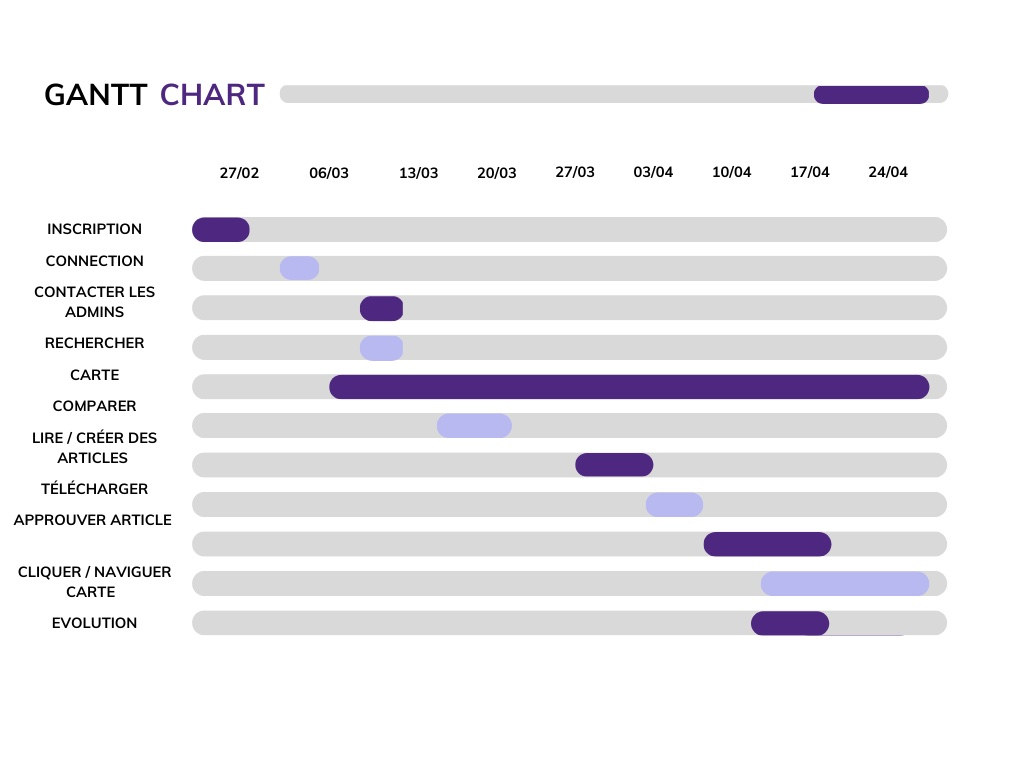
\includegraphics[width=1\textwidth]{images/gantt.jpg}
    \end{center}

\section{Modèle de la base de donnée}
\subsection{MCD}
    \begin{center}
        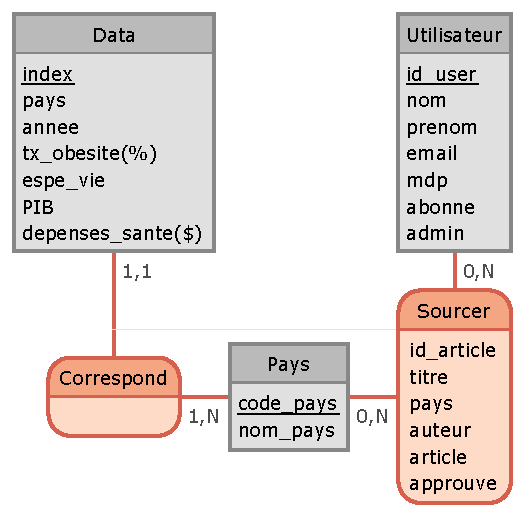
\includegraphics[width=0.4\textwidth]{images/Pays-2.pdf}
    \end{center}
\subsection{MOD}
\begin{itemize}
    \item DATA (idDonnée, année, txObésité, espéVie, pib, dépensesSanté, 
    codePays)
    \item PAYS (codePays, nomPays)
    \item UTILISATEUR (idUtil, email, mdp, abonné)
    \item SOURCER (codePays, idUtil, texte)
\end{itemize}

\section{Schéma de l'architecture}
    \begin{center}
        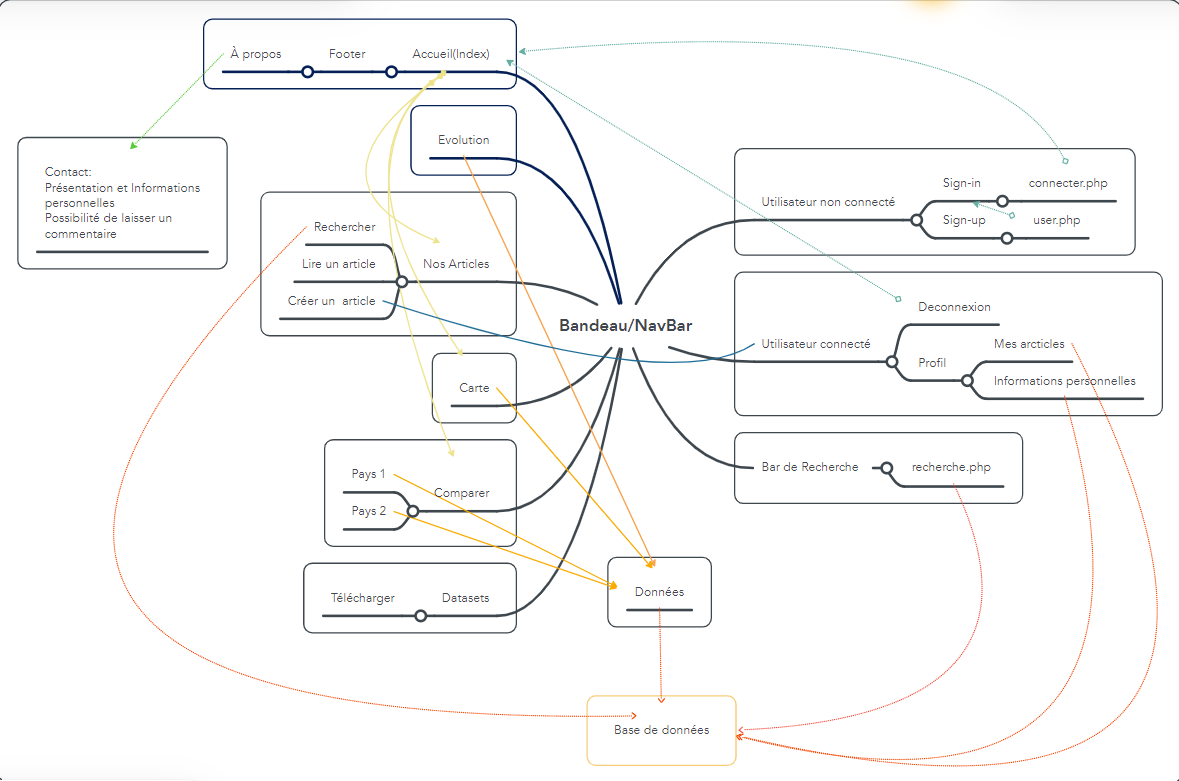
\includegraphics[width=1\textwidth]{images/architecture.png}
        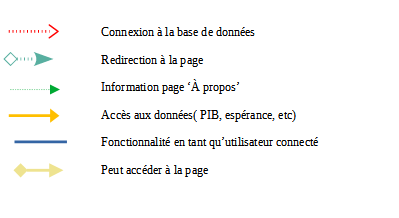
\includegraphics[width=0.5\textwidth]{images/legende_architecture.png}
    \end{center}

\chapter{Description fonctionnelle}
\section{Découvrez notre carte}

\chapter{Conclusion}
\section{Tableau des tâches}
\begin{tabular}{|c|c|c|c|c|c|c|}
\hline
Tâches & Audric & Malala & John & Axel & Ivan & Rachydah \\
\hline
MCD/MOD & 16\% & 16\% & 16\% & 16\% & 16\% & 16\%\\
\hline
Traitement des données & & & & & 100\% & \\
\hline
Front end & 40\% & & & & 60\% & \\
\hline
Back end & 80\% & & 15\% & 5\% & &\\
\hline
BDD online & & & & & 100\% & \\
\hline
Rapport & & 10\% & & 80\% & & 10\% \\
\hline
Diapos & & 80\% & & 20\% & & \\
\hline
Script soutenance & & & & 60\% & & 40\% \\
\hline
\end{tabular}

\section{Résumé des contributions}
 \begin{center}
        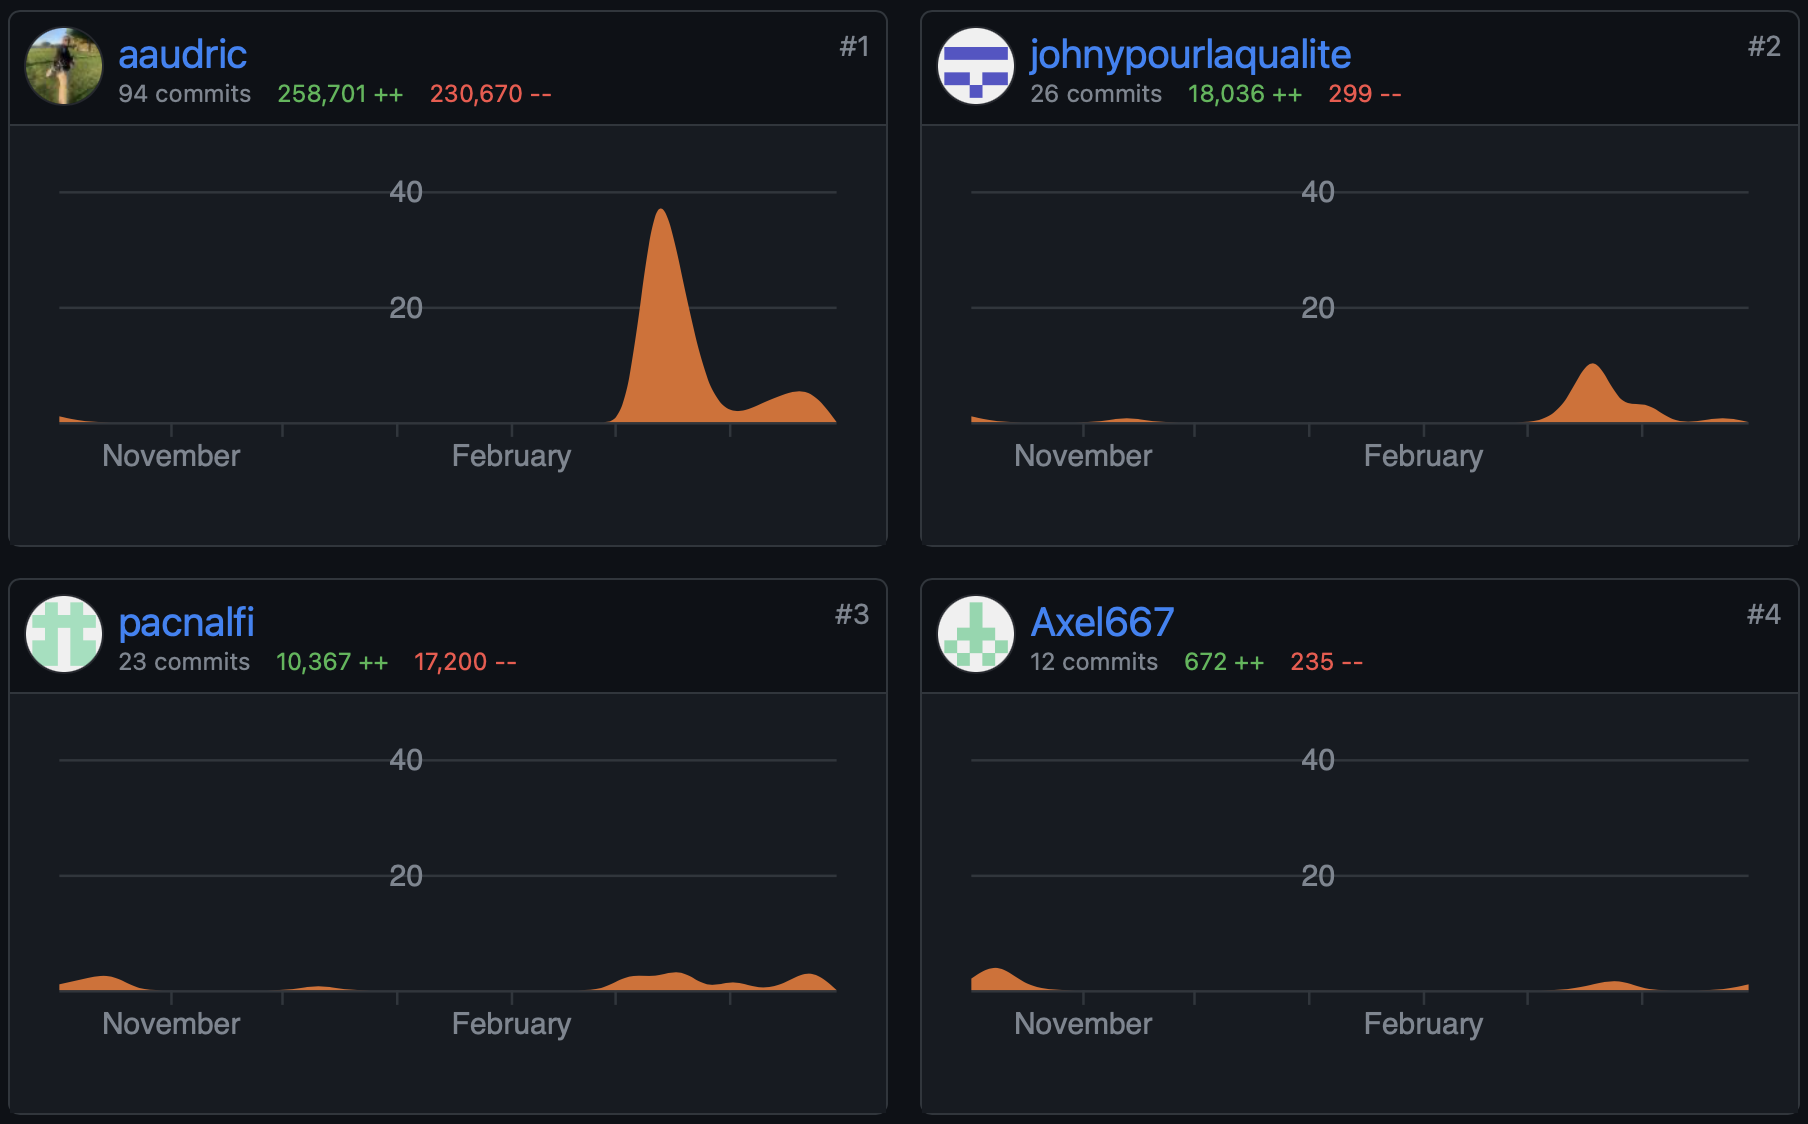
\includegraphics[width=1\textwidth]{images/contribution1.png}
        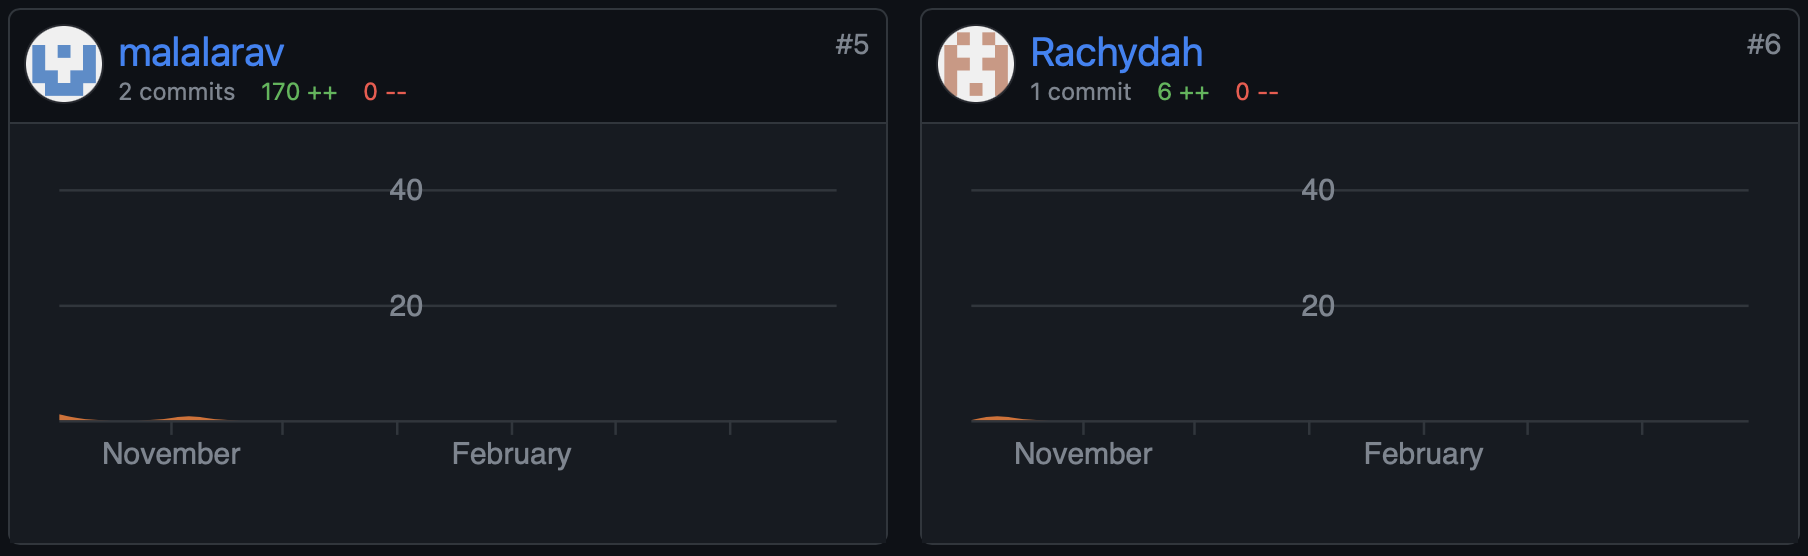
\includegraphics[width=1\textwidth]{images/contribution2.png}
\end{center}

\section{Difficultés rencontrées}
Nous n'avons pas rencontré de difficultés majeures pour la réalisation technique du projet mise à part au niveau de la carte. En effet, cette tâche a pris plus de temps que prévu car nous avions des difficultées à afficher les données sur la carte. \\

De plus, le passage en distanciel lors de la fermeture de l'université n'a pas aidé au bon développement du projet. Nous avons aussi eu besoin d'un petit temps d'adaptation pour nous familiariser avec git et github qui ont été des outils indispensables pour l'avancement du projet en groupe. Pour cela, nous avons su mettre en pratique les cours de gestion de projet du premier semestre. \\

Vers la fin du projet, il nous a aussi fallu prendre du recule sur le projet pour pouvoir se mettre à la place de l'utilsateur et corriger certains détails au niveau du front end pour le rendre plus ergonomique. 

\section{Conclusions générales et perspectives}
Malheureusement, l'hébergement du site n'a pas pu être réalisé car nous n'avons pas trouvé de solution optimale. Nous aurions aussi voulu rajouter la possibilité de mofidier un article mais nous avons manqué de temps. \\

Pour conclure, nous avons réussis à produire un site qui réponds à tout les objectifs que nous nous étions fixer. La réalisation de ce projet a été exigeante mais nous avons relevé ce défi. Nous avons pu mettre en pratique nos compétences en programmation web et nous sommes fières du résultat. 


\end{document}
